%!TEX root = ../../Systementwurf2.tex

\section{Implementierung von Komponente <C30>: Datenbank}

Die Datenbankkomponente dient zur Kommunikation mit dem Virtuoso Triplestore und dem Apache Lucene Index. Die Kommunikation mit den anderen Komponenten erfolgt eventbasiert mit Hilfe des Akka-Frameworks.

\subsection{Paket-/Klassendiagramm}

\begin{figure}[ht]
\centering
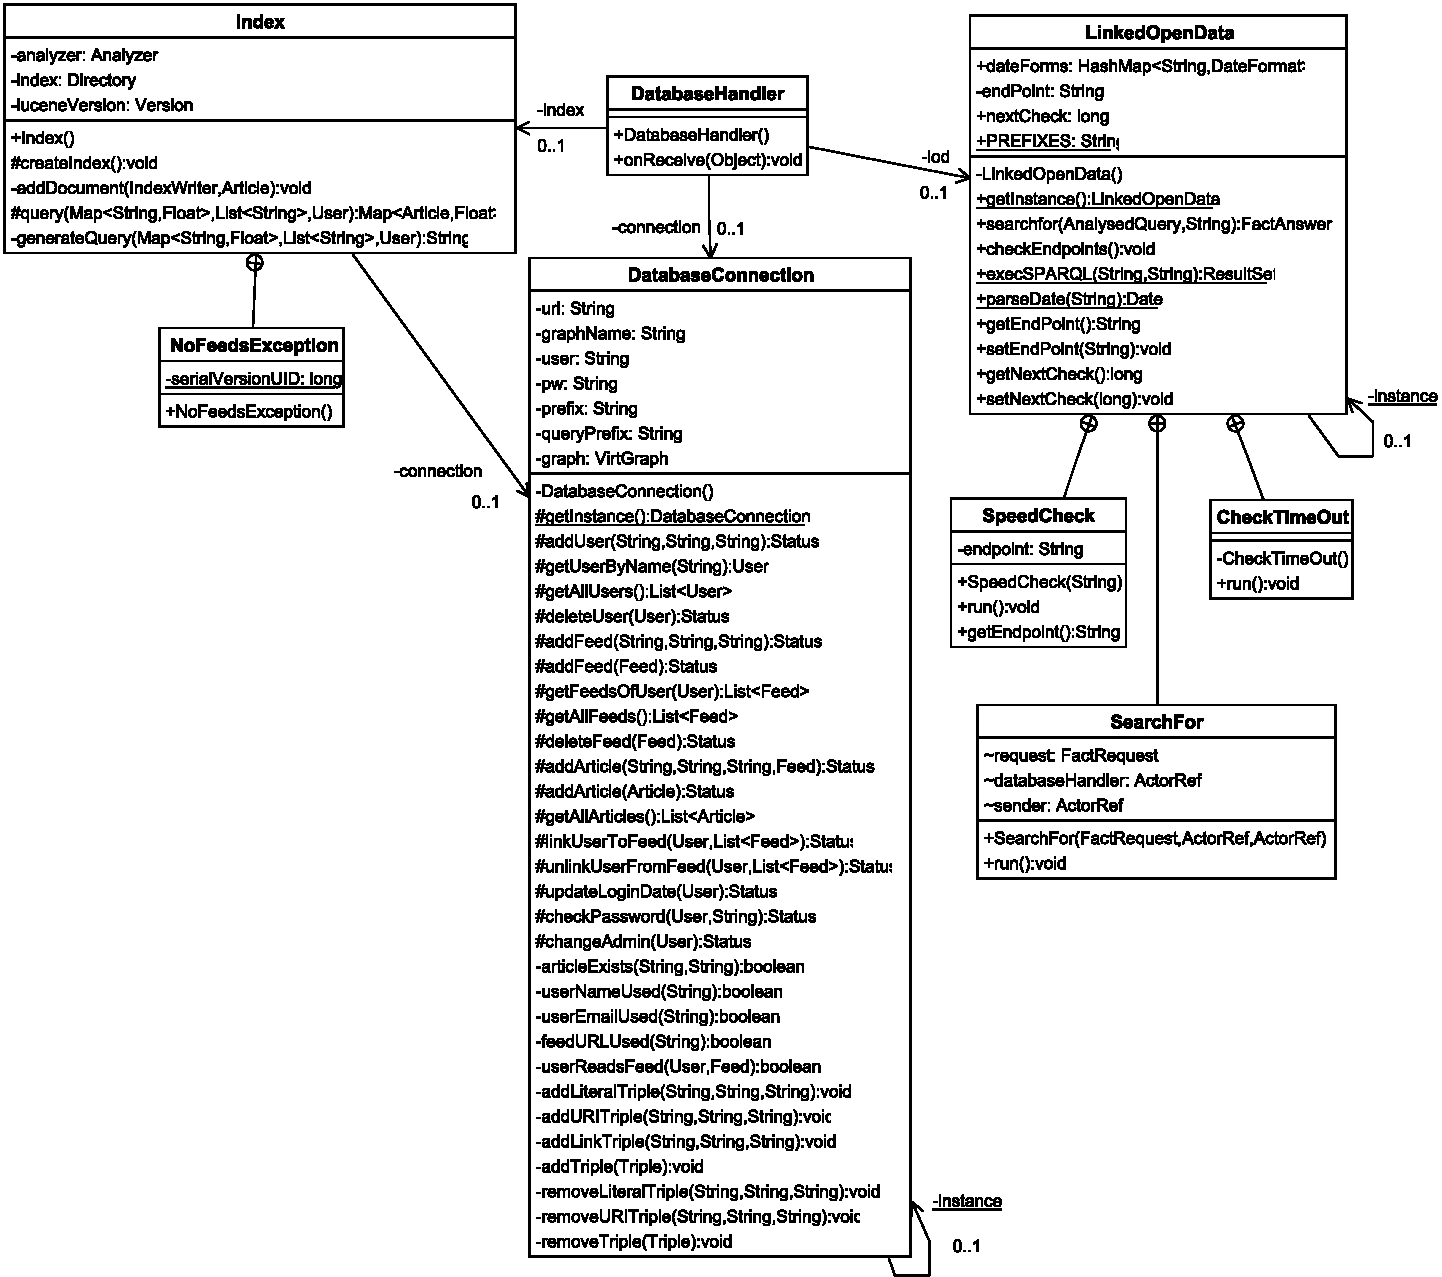
\includegraphics[width=1.03\textwidth]{Systementwurf/05_implementierungsentwurf/database}
\caption{Klassendiagramm für Komponente \ref{C30}}
\end{figure}

\subsection{Erläuterung}

Im Folgenden werden Attribute, Aufgaben und Kommunikationspartner für jede
Klasse der Datenbankkomponente kurz erläutert.

\begin{class}{10}{DatabaseHandler}
\item[Aufgabe]~\
Die DatabaseHandler-Klasse ist die Hauptklasse der Datenbankkomponente. Sie nimmt Anfragen der anderen Komponenten mittels der onReceive() Methode entgegen und sendet Antworten auf diese Anfragen.
\item[Attribute]~\
\begin{itemize}
  \item \texttt{connection}: Referenz auf den \textit{DatabaseConnection}-Singleton.
  \item \texttt{index}: Referenz auf ein \textit{Index}-Objekt.
  \item \texttt{lod}: Referenz auf den \textit{LinkedOpenData}-Singleton.
\end{itemize}
\item[Operationen]~\
\begin{itemize}
  \item \texttt{onReceive()}: nimmt Anfragen anderer Komponenten entgegen und beantwortet sie.
\end{itemize}
\item[Kommunikationspartner]~\
  \textit{DatabaseConnection}, \textit{Index}, \textit{LinkedOpenData}, \textit{Searcher}, \textit{CrawlerHandler}, \textit{ManagementHandler}
\end{class}

\begin{class}{20}{DatabaseConnection}
\item[Aufgabe]~\
Die DatabaseConnection-Klasse enthält die verschiedenen SPARQL-Queries an den Virtuoso-Triplestore.
\item[Attribute]~\
\begin{itemize}
  \item \texttt{instance}: Referenz auf den \textit{DatabaseConnection}-Singleton.
  \item \texttt{url}: URL unter der die Virtuoso-Datenbank erreicht werden kann.
  \item \texttt{graphName}: Name des RDF-Graphen auf dem gearbeitet wird.
  \item \texttt{user}: Virtuoso-Benutzername.
  \item \texttt{pw}: Virtuoso-Benutzerpasswort.
  \item \texttt{prefix}: Prefix für URI Graphenknoten.
  \item \texttt{queryPrefix}: Prefix für URI Graphenknoten in Queries.
  \item \texttt{graph}: Referenz auf den RDF-Graphen auf dem gearbeitet wird.
\end{itemize}
\item[Operationen]~\
\begin{itemize}
    \item \texttt{getInstance()}  Liefert die Singleton-Instanz.
    \item \texttt{addUser(String, String, String)} Legt einen neuen Benutzer in der Datenbank an.
    \item \texttt{getUserByName(String)} Liefert den Benutzer mit dem angegebenen Namen.
    \item \texttt{getAllUsers()} Liefert alle exisistierenden Benutzer.
    \item \texttt{deleteUser(User)} Löscht den angegebenen Benutzer.
    \item \texttt{addFeed(String, String, String)} Legt einen neuen Feed in der Datenbank an.
    \item \texttt{addFeed(Feed)} Legt einen neuen Feed in der Datenbank an.
    \item \texttt{getFeedsOfUser(User)} Liefert die Feeds, die der angegebene Benutzer abonniert hat.
    \item \texttt{getAllFeeds()} Liefert alle existierenden Feeds.
    \item \texttt{deleteFeed(Feed)} Löscht den angegebenen Feed.
    \item \texttt{addArticle(String, String, String, Feed)} Legt einen neuen Artikel in der Datenbank an.
    \item \texttt{addArticle(Article)} Legt einen neuen Artikel in der Datenbank an.
    \item \texttt{getallArticles()} Liefert alle existierenden Artikel.
    \item \texttt{linkUserToFeed(User, List<Feed>)} Verknüpft den angegebenen Benutzer mit den Feeds aus der Liste.
    \item \texttt{unlinkUserFromFeed(User, List<Feed>)} Löscht die Verknüpfungen zwischen dem angegebenen Benutzer und den Feeds aus der Liste.
    \item \texttt{updateLoginDate(User)} Ändert das Datum des letzten Logins des angegebenen Benutzers auf die momentane Zeit.
    \item \texttt{checkPassword(User, String)} Prüft, ob der angegebene Benutzer das angegebene Passwort verwendet.
    \item \texttt{changeAdmin(User)} Ändert den Admin-Status des angegebenen Benutzers.
    \item Hilfsfunktionen: Die Klasse enthält einige private Hilfsfunktionen, die hier nicht näher erläutert werden.
\end{itemize}
\item[Kommunikationspartner]~\
\textit{DatabaseHandler}, \textit{Index}
\end{class}

\begin{class}{30}{Index}
\item[Aufgabe]~\
Die Index-Klasse verwaltet den Apache Lucene Volltextindex.
\item[Attribute]~\
\begin{itemize}
  \item \texttt{analyzer}: Legt fest, welcher Lucene-Analyzer verwendet wird.
  \item \texttt{index}: Ordner, in dem sich der Index im Dateisystem befindet.
  \item \texttt{luceneVersion}: Legt fest, welche Lucene Version verwendet wird.
  \item \texttt{connection}: Referenz auf den \textit{DatabaseConnection}-Singleton.
\end{itemize}
\item[Operationen]~\
\begin{itemize}
    \item \texttt{createIndex()}  Schreibt den Index neu. Dies ist nach jedem Durchlauf des Crawlers notwendig.
    \item \texttt{addDocument(IndexWriter, Article)} Hilfsfunktion von \texttt{createIndex()}.
    \item \texttt{query(Map<String, Float>, List<String>, User)} Stellt einen Query an den Index.
    \item \texttt{generateQuery(Map<String, Float>, List<String>, User)} Hilfsfunktion von\\ \texttt{query(Map<String, Float>, List<String>, User)}.
\end{itemize}
\item[Kommunikationspartner]~\
\textit{DatabaseHandler}, \textit{DataBaseConnection}
\end{class}

\begin{class}{30}{NoFeedsException}
\item[Aufgabe]~\
Intern verwendete Exception, die auftritt, wenn ein Benutzer keine Feeds aboniert hat.
\item[Attribute]~\ keine
\item[Operationen]~\ keine
\item[Kommunikationspartner]~\ keine
\end{class}
